\chapter{Segunda aproximación Greedy}
% Para resolver los problemas de la primera aproximación realizada, se ha desarrollado un segundo algoritmo greedy. A esta segunda aproximación se le ha añadido un algoritmo previo que sirve para hacer la estructura del horario y cuyo objetivo es minimizar la ocupación de los laboratorios de prácticas.

A raíz de los problemas vistos en la versión anterior, se optó por modificar lo desarrollado hasta ahora y hacer una segunda versión del algoritmo greedy capaz de solventar estos problemas y mejorar la calidad de las soluciones. 

En esta segunda aproximación se realizan varias cosas:

\begin{enumerate}
  \item Simplificación del modelo: se reestructurarán las clases, eliminando elementos innecesarios que aumentan la complejidad del algoritmo y por tanto la complejidad del problema. 
  \item Añadir un paso previo al algoritmo: este paso previo consiste en calcular la estructura básica del horario, preasignando celdas como celdas de teoría o de prácticas, independientemente de la asignatura que se vaya a asignar para facilitar la composición del horario. Más adelante se verá esto con más detalle.
\end{enumerate}

\section{Simplificación del modelo}

Una de las simplificaciones más importantes que se ha hecho del modelo es la eliminación total de los materiales que tiene cada aula y que necesita cada asignatura. Esto aunque pueda parecer muy simple, simplifica enormemente el modelo. 

Esta modificación no se hace así sin más. En vez de haber una lista de materiales posibles que ofrecen las aulas y materiales que necesitan las asignaturas, para después buscar posibles aulas haciendo una intersección, se cambia esto por una lista de aulas en las que se puede impartir una asignatura y se elige una entre las posibles que esté libre. 

Es decir, para aquellas asignaturas que tengan una fuerte restricción de materiales, se les asignará sólo las aulas en las que puedan ser impartidas, y para el resto de asignaturas, se les asignará un aula que esté libre en ese momento entre las distintas aulas de prácticas de las que dispone el centro

Esto sucede en el centro para asignaturas como \textit{Fundamentos Físicos y Tecnológicos}, que necesita aulas con material electrónico, o asignaturas con restricciones más fuertes aún como son \textit{Tecnología y Organización de Computadores} y \textit{Fundamentos de Redes}, que en nuestro centro, no tienen más remedio que ir asignadas al aula 3.10 y 2.7 respectivamente, por las restricciones tan fuertes de materiales que tienen.

Con esto, podemos eliminar los atributos que se usan para almacenar los materiales que necesita cada asignatura, y los materiales de los que dispone cada aula de prácticas, quedando algo como lo que podemos ver en la \hyperref[clases3]{Figura \ref*{clases3}}.

\begin{figure}[H]
  % Graphic for TeX using PGF
% Title: /home/braulio/PycharmProjects/TFG/doc/clases.dia
% Creator: Dia v0.97.3
% CreationDate: Mon Sep  4 20:42:15 2017
% For: braulio
% \usepackage{tikz}
% The following commands are not supported in PSTricks at present
% We define them conditionally, so when they are implemented,
% this pgf file will use them.
\ifx\du\undefined
  \newlength{\du}
\fi
\setlength{\du}{15\unitlength}
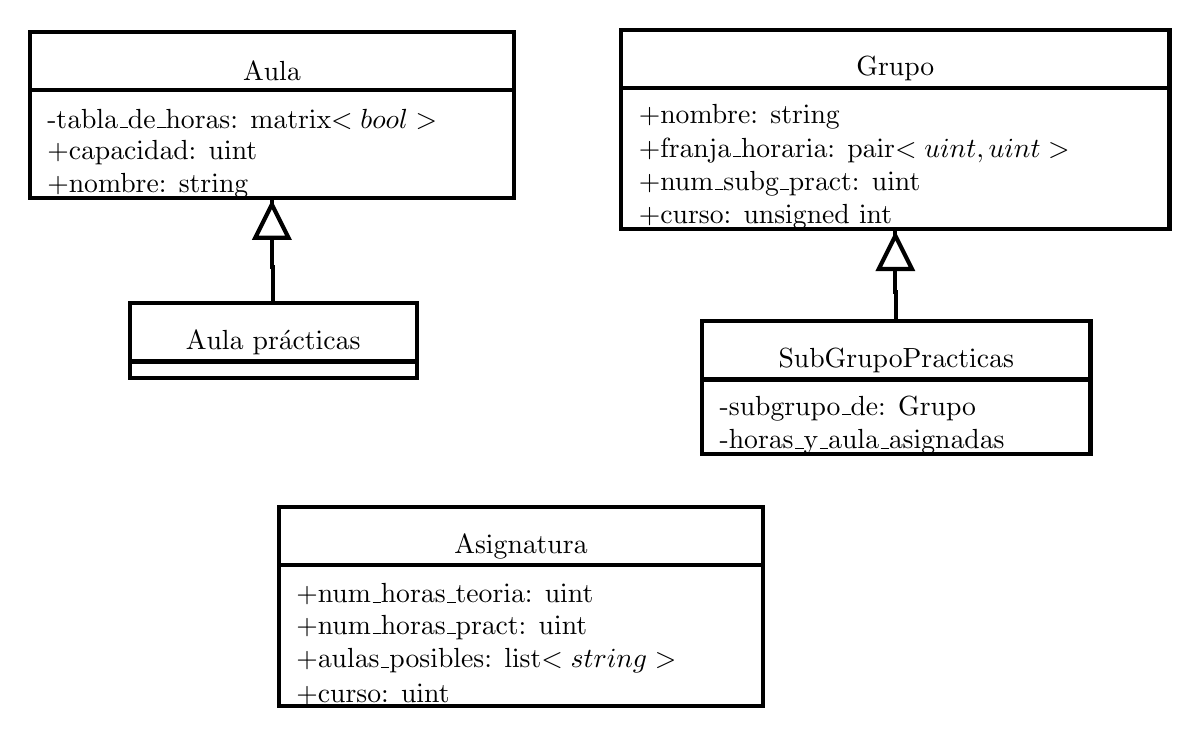
\begin{tikzpicture}
\pgftransformxscale{1.000000}
\pgftransformyscale{-1.000000}
\definecolor{dialinecolor}{rgb}{0.000000, 0.000000, 0.000000}
\pgfsetstrokecolor{dialinecolor}
\definecolor{dialinecolor}{rgb}{1.000000, 1.000000, 1.000000}
\pgfsetfillcolor{dialinecolor}
\pgfsetlinewidth{0.100000\du}
\pgfsetdash{}{0pt}
\definecolor{dialinecolor}{rgb}{1.000000, 1.000000, 1.000000}
\pgfsetfillcolor{dialinecolor}
\fill (12.350000\du,4.800000\du)--(12.350000\du,6.200000\du)--(24.015000\du,6.200000\du)--(24.015000\du,4.800000\du)--cycle;
\definecolor{dialinecolor}{rgb}{0.000000, 0.000000, 0.000000}
\pgfsetstrokecolor{dialinecolor}
\draw (12.350000\du,4.800000\du)--(12.350000\du,6.200000\du)--(24.015000\du,6.200000\du)--(24.015000\du,4.800000\du)--cycle;
% setfont left to latex
\definecolor{dialinecolor}{rgb}{0.000000, 0.000000, 0.000000}
\pgfsetstrokecolor{dialinecolor}
\node at (18.182500\du,5.750000\du){Aula};
\definecolor{dialinecolor}{rgb}{1.000000, 1.000000, 1.000000}
\pgfsetfillcolor{dialinecolor}
\fill (12.350000\du,6.200000\du)--(12.350000\du,8.800000\du)--(24.015000\du,8.800000\du)--(24.015000\du,6.200000\du)--cycle;
\definecolor{dialinecolor}{rgb}{0.000000, 0.000000, 0.000000}
\pgfsetstrokecolor{dialinecolor}
\draw (12.350000\du,6.200000\du)--(12.350000\du,8.800000\du)--(24.015000\du,8.800000\du)--(24.015000\du,6.200000\du)--cycle;
% setfont left to latex
\definecolor{dialinecolor}{rgb}{0.000000, 0.000000, 0.000000}
\pgfsetstrokecolor{dialinecolor}
\node[anchor=west] at (12.500000\du,6.900000\du){-tabla\_de\_horas: matrix$<bool>$};
% setfont left to latex
\definecolor{dialinecolor}{rgb}{0.000000, 0.000000, 0.000000}
\pgfsetstrokecolor{dialinecolor}
\node[anchor=west] at (12.500000\du,7.700000\du){+capacidad: uint};
% setfont left to latex
\definecolor{dialinecolor}{rgb}{0.000000, 0.000000, 0.000000}
\pgfsetstrokecolor{dialinecolor}
\node[anchor=west] at (12.500000\du,8.500000\du){+nombre: string};
\pgfsetlinewidth{0.100000\du}
\pgfsetdash{}{0pt}
\definecolor{dialinecolor}{rgb}{1.000000, 1.000000, 1.000000}
\pgfsetfillcolor{dialinecolor}
\fill (14.756600\du,11.342000\du)--(14.756600\du,12.742000\du)--(21.669100\du,12.742000\du)--(21.669100\du,11.342000\du)--cycle;
\definecolor{dialinecolor}{rgb}{0.000000, 0.000000, 0.000000}
\pgfsetstrokecolor{dialinecolor}
\draw (14.756600\du,11.342000\du)--(14.756600\du,12.742000\du)--(21.669100\du,12.742000\du)--(21.669100\du,11.342000\du)--cycle;
% setfont left to latex
\definecolor{dialinecolor}{rgb}{0.000000, 0.000000, 0.000000}
\pgfsetstrokecolor{dialinecolor}
\node at (18.212850\du,12.292000\du){Aula prácticas};
\definecolor{dialinecolor}{rgb}{1.000000, 1.000000, 1.000000}
\pgfsetfillcolor{dialinecolor}
\fill (14.756600\du,12.742000\du)--(14.756600\du,13.142000\du)--(21.669100\du,13.142000\du)--(21.669100\du,12.742000\du)--cycle;
\definecolor{dialinecolor}{rgb}{0.000000, 0.000000, 0.000000}
\pgfsetstrokecolor{dialinecolor}
\draw (14.756600\du,12.742000\du)--(14.756600\du,13.142000\du)--(21.669100\du,13.142000\du)--(21.669100\du,12.742000\du)--cycle;
\pgfsetlinewidth{0.100000\du}
\pgfsetdash{}{0pt}
\pgfsetmiterjoin
\pgfsetbuttcap
{
\definecolor{dialinecolor}{rgb}{0.000000, 0.000000, 0.000000}
\pgfsetfillcolor{dialinecolor}
% was here!!!
\definecolor{dialinecolor}{rgb}{0.000000, 0.000000, 0.000000}
\pgfsetstrokecolor{dialinecolor}
\draw (18.182500\du,8.850250\du)--(18.182500\du,10.470893\du)--(18.212850\du,10.470893\du)--(18.212850\du,11.291536\du);
}
\definecolor{dialinecolor}{rgb}{0.000000, 0.000000, 0.000000}
\pgfsetstrokecolor{dialinecolor}
\draw (18.182500\du,9.762054\du)--(18.182500\du,10.470893\du)--(18.212850\du,10.470893\du)--(18.212850\du,11.291536\du);
\pgfsetmiterjoin
\definecolor{dialinecolor}{rgb}{1.000000, 1.000000, 1.000000}
\pgfsetfillcolor{dialinecolor}
\fill (18.582500\du,9.762054\du)--(18.182500\du,8.962054\du)--(17.782500\du,9.762054\du)--cycle;
\pgfsetlinewidth{0.100000\du}
\pgfsetdash{}{0pt}
\pgfsetmiterjoin
\definecolor{dialinecolor}{rgb}{0.000000, 0.000000, 0.000000}
\pgfsetstrokecolor{dialinecolor}
\draw (18.582500\du,9.762054\du)--(18.182500\du,8.962054\du)--(17.782500\du,9.762054\du)--cycle;
% setfont left to latex
\pgfsetlinewidth{0.100000\du}
\pgfsetdash{}{0pt}
\definecolor{dialinecolor}{rgb}{1.000000, 1.000000, 1.000000}
\pgfsetfillcolor{dialinecolor}
\fill (26.600000\du,4.750000\du)--(26.600000\du,6.150000\du)--(39.805000\du,6.150000\du)--(39.805000\du,4.750000\du)--cycle;
\definecolor{dialinecolor}{rgb}{0.000000, 0.000000, 0.000000}
\pgfsetstrokecolor{dialinecolor}
\draw (26.600000\du,4.750000\du)--(26.600000\du,6.150000\du)--(39.805000\du,6.150000\du)--(39.805000\du,4.750000\du)--cycle;
% setfont left to latex
\definecolor{dialinecolor}{rgb}{0.000000, 0.000000, 0.000000}
\pgfsetstrokecolor{dialinecolor}
\node at (33.202500\du,5.700000\du){Grupo};
\definecolor{dialinecolor}{rgb}{1.000000, 1.000000, 1.000000}
\pgfsetfillcolor{dialinecolor}
\fill (26.600000\du,6.150000\du)--(26.600000\du,9.550000\du)--(39.805000\du,9.550000\du)--(39.805000\du,6.150000\du)--cycle;
\definecolor{dialinecolor}{rgb}{0.000000, 0.000000, 0.000000}
\pgfsetstrokecolor{dialinecolor}
\draw (26.600000\du,6.150000\du)--(26.600000\du,9.550000\du)--(39.805000\du,9.550000\du)--(39.805000\du,6.150000\du)--cycle;
% setfont left to latex
\definecolor{dialinecolor}{rgb}{0.000000, 0.000000, 0.000000}
\pgfsetstrokecolor{dialinecolor}
\node[anchor=west] at (26.750000\du,6.850000\du){+nombre: string};
% setfont left to latex
\definecolor{dialinecolor}{rgb}{0.000000, 0.000000, 0.000000}
\pgfsetstrokecolor{dialinecolor}
\node[anchor=west] at (26.750000\du,7.650000\du){+franja\_horaria: pair$<uint, uint>$};
% setfont left to latex
\definecolor{dialinecolor}{rgb}{0.000000, 0.000000, 0.000000}
\pgfsetstrokecolor{dialinecolor}
\node[anchor=west] at (26.750000\du,8.450000\du){+num\_subg\_pract: uint};
% setfont left to latex
\definecolor{dialinecolor}{rgb}{0.000000, 0.000000, 0.000000}
\pgfsetstrokecolor{dialinecolor}
\node[anchor=west] at (26.750000\du,9.250000\du){+curso: unsigned int};
\pgfsetlinewidth{0.100000\du}
\pgfsetdash{}{0pt}
\definecolor{dialinecolor}{rgb}{1.000000, 1.000000, 1.000000}
\pgfsetfillcolor{dialinecolor}
\fill (18.350000\du,16.250000\du)--(18.350000\du,17.650000\du)--(30.015000\du,17.650000\du)--(30.015000\du,16.250000\du)--cycle;
\definecolor{dialinecolor}{rgb}{0.000000, 0.000000, 0.000000}
\pgfsetstrokecolor{dialinecolor}
\draw (18.350000\du,16.250000\du)--(18.350000\du,17.650000\du)--(30.015000\du,17.650000\du)--(30.015000\du,16.250000\du)--cycle;
% setfont left to latex
\definecolor{dialinecolor}{rgb}{0.000000, 0.000000, 0.000000}
\pgfsetstrokecolor{dialinecolor}
\node at (24.182500\du,17.200000\du){Asignatura};
\definecolor{dialinecolor}{rgb}{1.000000, 1.000000, 1.000000}
\pgfsetfillcolor{dialinecolor}
\fill (18.350000\du,17.650000\du)--(18.350000\du,21.050000\du)--(30.015000\du,21.050000\du)--(30.015000\du,17.650000\du)--cycle;
\definecolor{dialinecolor}{rgb}{0.000000, 0.000000, 0.000000}
\pgfsetstrokecolor{dialinecolor}
\draw (18.350000\du,17.650000\du)--(18.350000\du,21.050000\du)--(30.015000\du,21.050000\du)--(30.015000\du,17.650000\du)--cycle;
% setfont left to latex
\definecolor{dialinecolor}{rgb}{0.000000, 0.000000, 0.000000}
\pgfsetstrokecolor{dialinecolor}
\node[anchor=west] at (18.500000\du,18.350000\du){+num\_horas\_teoria: uint};
% setfont left to latex
\definecolor{dialinecolor}{rgb}{0.000000, 0.000000, 0.000000}
\pgfsetstrokecolor{dialinecolor}
\node[anchor=west] at (18.500000\du,19.150000\du){+num\_horas\_pract: uint};
% setfont left to latex
\definecolor{dialinecolor}{rgb}{0.000000, 0.000000, 0.000000}
\pgfsetstrokecolor{dialinecolor}
\node[anchor=west] at (18.500000\du,19.950000\du){+aulas\_posibles: list$<string>$};
% setfont left to latex
\definecolor{dialinecolor}{rgb}{0.000000, 0.000000, 0.000000}
\pgfsetstrokecolor{dialinecolor}
\node[anchor=west] at (18.500000\du,20.750000\du){+curso: uint};
\pgfsetlinewidth{0.100000\du}
\pgfsetdash{}{0pt}
\definecolor{dialinecolor}{rgb}{1.000000, 1.000000, 1.000000}
\pgfsetfillcolor{dialinecolor}
\fill (28.547000\du,11.775000\du)--(28.547000\du,13.175000\du)--(37.902000\du,13.175000\du)--(37.902000\du,11.775000\du)--cycle;
\definecolor{dialinecolor}{rgb}{0.000000, 0.000000, 0.000000}
\pgfsetstrokecolor{dialinecolor}
\draw (28.547000\du,11.775000\du)--(28.547000\du,13.175000\du)--(37.902000\du,13.175000\du)--(37.902000\du,11.775000\du)--cycle;
% setfont left to latex
\definecolor{dialinecolor}{rgb}{0.000000, 0.000000, 0.000000}
\pgfsetstrokecolor{dialinecolor}
\node at (33.224500\du,12.725000\du){SubGrupoPracticas};
\definecolor{dialinecolor}{rgb}{1.000000, 1.000000, 1.000000}
\pgfsetfillcolor{dialinecolor}
\fill (28.547000\du,13.175000\du)--(28.547000\du,14.975000\du)--(37.902000\du,14.975000\du)--(37.902000\du,13.175000\du)--cycle;
\definecolor{dialinecolor}{rgb}{0.000000, 0.000000, 0.000000}
\pgfsetstrokecolor{dialinecolor}
\draw (28.547000\du,13.175000\du)--(28.547000\du,14.975000\du)--(37.902000\du,14.975000\du)--(37.902000\du,13.175000\du)--cycle;
% setfont left to latex
\definecolor{dialinecolor}{rgb}{0.000000, 0.000000, 0.000000}
\pgfsetstrokecolor{dialinecolor}
\node[anchor=west] at (28.697000\du,13.875000\du){-subgrupo\_de: Grupo};
% setfont left to latex
\definecolor{dialinecolor}{rgb}{0.000000, 0.000000, 0.000000}
\pgfsetstrokecolor{dialinecolor}
\node[anchor=west] at (28.697000\du,14.675000\du){-horas\_y\_aula\_asignadas};
\pgfsetlinewidth{0.100000\du}
\pgfsetdash{}{0pt}
\pgfsetmiterjoin
\pgfsetbuttcap
{
\definecolor{dialinecolor}{rgb}{0.000000, 0.000000, 0.000000}
\pgfsetfillcolor{dialinecolor}
% was here!!!
\definecolor{dialinecolor}{rgb}{0.000000, 0.000000, 0.000000}
\pgfsetstrokecolor{dialinecolor}
\draw (33.202500\du,9.600299\du)--(33.202500\du,11.062448\du)--(33.224500\du,11.062448\du)--(33.224500\du,11.724597\du);
}
\definecolor{dialinecolor}{rgb}{0.000000, 0.000000, 0.000000}
\pgfsetstrokecolor{dialinecolor}
\draw (33.202500\du,10.512102\du)--(33.202500\du,11.062448\du)--(33.224500\du,11.062448\du)--(33.224500\du,11.724597\du);
\pgfsetmiterjoin
\definecolor{dialinecolor}{rgb}{1.000000, 1.000000, 1.000000}
\pgfsetfillcolor{dialinecolor}
\fill (33.602500\du,10.512102\du)--(33.202500\du,9.712102\du)--(32.802500\du,10.512102\du)--cycle;
\pgfsetlinewidth{0.100000\du}
\pgfsetdash{}{0pt}
\pgfsetmiterjoin
\definecolor{dialinecolor}{rgb}{0.000000, 0.000000, 0.000000}
\pgfsetstrokecolor{dialinecolor}
\draw (33.602500\du,10.512102\du)--(33.202500\du,9.712102\du)--(32.802500\du,10.512102\du)--cycle;
% setfont left to latex
\end{tikzpicture}

  \caption{Nueva estructura de clases y atributos.}
  \label{clases3}
\end{figure}

Esto tiene una serie de consecuencias y una de ellas es que el espacio de búsqueda para realizar una asignación de aulas crece, por lo que el problema, en la teoría, se dificulta. En la práctica sucede que al tener menos restricciones, podemos simplemente asignar una asignatura a cualquier aula que esté libre, siempre y cuando no se infrinja la condición de que las asignaturas con más restricciones de aulas como las que hemos visto anteriormente tengan asignadas las aulas esperadas.

Otra consecuencia derivada de esta decisión es que el espacio en memoria que necesita la máquina para ejecutar el algoritmo se reduce enormemente al no tener que almacenar listas de materiales para todas y cada una de las asignaturas, al igual que con las distintas aulas. Esto supone que máquinas con muchas menos prestaciones que las máquinas en las que se ha desarrollado el proyecto, puedan ejecutar el algoritmo sin problemas al necesitar menos memoria. También se mejora el tiempo de ejecución, ya que no se producen tantos accesos a memoria, tanto para consultar como para escribir a las distintas listas de materiales, etc.

\section{Preasignación de horas}
Ante la aparición de estos problemas en la primera versión del algoritmo, decidimos volver a analizar el problema y reestructurar los algoritmos, obteniendo una nueva versión del algoritmo greedy. Para llevar a cabo esta tarea, tuvimos varias reuniones con Dº Jesús García Miranda, para hablar sobre los problemas que tenía la primera versión, y discutir nuevas soluciones a este problema. 

Una de las soluciones principales que nos dio, fue la de generar una estructura de datos auxiliar en la que se calculará una estructura preliminar del horario. En ella se asignarán qué casillas de las que hay en el horario se clasifican como clases de teoría y cuáles como clases de prácticas. Esto se hace con el fin de evitar una saturación en las aulas del centro, haciendo que si un grupo $x$ tiene una clase de teoría en el momento $(d, h)$, un grupo $x'$ tendrá en ese momento clase de prácticas, optimizando de esta forma el espacio.

Esta preasignación en el horario se hace sólo teniendo en cuenta el número de horas de teoría y prácticas totales que tiene un grupo concreto para un curso, en vez de ir mirando asignatura por asignatura. De esta forma se obtiene una visión mucho más global del problema y se empieza a construir una buena solución desde el momento inicial del algoritmo, lo que hace que sea más fácil obtener buenas soluciones, a pesar de que esto suponga también limitar el espacio de búsqueda del problema. El objetivo de esta fase es simplemente minimizar la ocupación de los laboratorios de prácticas y teoría, evitando una saturación de las aulas del centro y optimizar los espacios de este.

A su vez, esto nos permite simplificar mucho el algoritmo, porque aunque hay que añadir una fase más al algoritmo, las fases siguientes sólo tienen que completar ``el puzzle con pistas'' que nos ha dejado esta fase, simplificando tanto la estructura de los algoritmos, tiempos de ejecución, consumo de memoria, etc.

Por sencillez, se ha decidido que este algoritmo sólo calcula una franja, en vez de las dos para que el algoritmo sea más simple. Esta franja se decide mediante un parámetro en el que se establece la franja horaria (mañana o tarde). Es por esto, por lo que deben filtrarse los grupos y trabajar con aquellos que pertenezcan al turno que se está calculando. Una vez filtrados estos grupos, el algoritmo irá calculando la estructura para cada uno de los cursos que corresponden.

El algoritmo antes de comenzar el bucle principal, realiza una serie de cálculos. Para empezar, calcula el número total de horas de teoría y prácticas que tiene para cada curso. Además de esto, hay que calcular el número de horas totales libres de laboratorio que hay, para comprobar si en algún momento en el horario habrá grupos que tengan en el mismo instante de tiempo prácticas a la vez. Por ejemplo, si los laboratorios están abiertos cinco días a la semana y cuatro horas al día tendríamos un total de 20 horas. Como cada turno de prácticas tiene dos horas, nos quedarían un total de diez turnos de prácticas por asignar. Si, por ejemplo, tuviésemos que asignar doce turnos de prácticas, tendríamos que elegir de forma aleatoria dos turnos de prácticas que se repetirían. Debe ser de forma aleatoria para que los turnos ``repetidos'' no coincidan en los distintos cursos y se saturen los laboratorios un día en concreto.

Después, el algoritmo empieza a iterar sobre cada grupo de ese curso y va asignando horas de prácticas y teoría en los huecos ``libres''. Para saber qué huecos están libres se usa una matriz auxiliar que registra qué horas son de prácticas en cada curso.

\subsection{Pseudocódigo del algoritmo}
El siguiente pseudocódigo refleja de forma más clara el funcionamiento de este algoritmo:

\begin{pseudocode}{GreedyEstructura}{turno}
\label{greedyestructura}
filtro\_grupos \GETS \CALL{FiltrarGrupos}{turno}\\
principio \GETS \CALL{ComienzoFranja}{turno}\\
final \GETS \CALL{FinalFranja}{turno}\\
\FOREACH curso \in cursos \DO
\BEGIN
    filtro\_cursos \GETS \CALL{FiltrarGruposCurso}{curso, filtro\_grupos}\\
    h\_lab \GETS \CALL{CalcularHorasPracticasCurso}{curso}\\
    h\_week \GETS dias\_semana \cdot n\_turnos\\

    \IF h\_lab > h\_week \THEN
	    	dias\_rep \GETS \CALL{CalcularTurnosRepetidos}{ }
    \ELSE 
      dias\_rep \GETS \emptyset\\

   	tabla\_lab \GETS \CALL{Matriz}{dias\_semana, n\_turnos, value=False}\\

   	\FOREACH g \in filtro\_cursos \DO
   	\BEGIN
   		teoria \GETS \CALL{CalcularHorasTeoria}{g}\\
   		lab \GETS \CALL{CalcularHorasLab}{g}\\

   		\FOR hora \GETS 0 \TO final; i+=2 \DO
   		\BEGIN
   		   \FOR dia \in SEMANA \DO
           \BEGIN
                \IF \NOT tabla\_lab[hora, dia] \AND lab \ge 2 \THEN
                \BEGIN
                    \CALL{AsignarEstructura}{hora, dia, L}\\
                    tabla\_lab[hora, dia] = True\\
                    tabla\_lab[hora + 1, dia] = True\\
                    lab \GETS lab - 2\\
                \END
                \ELSEIF tabla\_lab[hora, dia] \AND lab \ge 2 \AND (dia, hora) \in dias\_rep \THEN
                \BEGIN
                    \CALL{delete}{dias\_rep(dia, hora)}\\
                    \CALL{AsignarEstructura}{hora, dia, L}\\
                    lab \GETS lab - 2\\
                \END
                \ELSEIF tabla\_lab[hora, dia] \AND teoria \ge 2 \THEN
                \BEGIN
                    \CALL{AsignarEstructura}{hora, dia, T}\\
                    teoria \GETS teoria - 2\\
                \END
                \ELSEIF teoria \ge 2 \THEN
                \BEGIN
                    \CALL{AsignarEstructura}{hora, dia, T}\\
                    teoria \GETS teoria - 2\\
                \END
                \ELSEIF lab \ge 2 \THEN
                \BEGIN
                    \CALL{AsignarEstructura}{hora, dia, L}\\
                    lab \GETS lab - 2\\
                \END
                \ELSEIF teoria = 1 \THEN
                \BEGIN
                  \CALL{AsignarEstructura}{hora, dia, T}\\
                  teoria \GETS teoria - 1\\
                \END
                \ELSEIF lab = 1 \THEN
                \BEGIN
                  \CALL{AsignarEstructura}{hora, dia, L}\\
                  lab \GETS lab - 1\\
                \END
                \ELSE \CALL{break}{}
           \END
   		\END
   	\END
\END
\end{pseudocode}

El algoritmo comienza filtrando los grupos según el turno que se esté calculando, además de caclcular el punto de partida y final para el bucle interno en función del turno, para no tener que estar constantemente calculándolo. Una vez pasado esto, pasamos al bucle principal.

Dentro del bucle principal, lo que hace el algoritmo es calcular el número de horas de prácticas que tiene el grupo y el número de horas totales que hay en una semana. En caso de que las horas de prácticas del grupo sean mayores que las que hay disponibles para una asignatura, se escogerá un día aleatorio de la semana en el que se va a repetir un turno.

\section{Asignación de horas de teoría}
Esta segunda versión del algoritmo de asignación de horas de teoría utiliza como base la estructura hecha por el algoritmo de preasignación. Así, sólo tiene permitido asignar horas en los huecos que estén marcados como \texttt{T} en la matriz de estructura. Usando esto como base y un diccionario con las horas por asignar de cada asignatura, el algoritmo distingue varios casos diferentes:

\begin{enumerate}[---]
  \item Si la hora actual no se corresponde a una de teoría en la matriz de estructura, el algoritmo no hace nada.
  \item Si la hora actual sí es de teoría y además la asignatura a asignar tiene más de dos horas pendientes por asignar, se crea un bloque de dos horas con dicha asignatura.
  \item Si la hora actual sí es de teoría pero la asignatura a asignar sólo tiene una hora más por asignar, el algoritmo trata de buscar otra con la que hacer un bloque de dos. En el caso de no existir, se asignaría esa hora únicamente.
\end{enumerate}

Cuando a una asignatura no le quedan más horas por asignar, se elimina automáticamente de la lista de asignaturas por asignar. El algoritmo pasa al siguiente grupo cuando dicha lista se queda vacía.

\subsection{Comparación con la primera versión}
En comparación con la primera versión, hay bastantes cosas que hemos mejorado:

\begin{enumerate}[$\bullet$]
  \item En la versión anterior, si no se conseguía hacer un bloque de dos con dos horas sueltas, el algoritmo o bien ciclaba o bien dejaba huecos en el horario, dando lugar a una estructura no deseada.
  \item En consecuencia, el algoritmo es más rápido que el anterior desarrollado.
  \item Usando el algoritmo de preasignación, hemos conseguido que el código sea mucho más sencillo y legible.
  \item También, el algoritmo ha perdido esa alta diversidad que tenía la versión original puesto que en la nueva versión se ha acotado mucho la estructura del algoritmo y el espacio de búsqueda.
\end{enumerate}

En conclusión, aunque el algoritmo haya perdido su diversidad original, hemos ganado tanto en eficiencia como en calidad.

\subsection{Pseudocódigo del algoritmo}
El siguiente pseudocódigo refleja de forma más clara el funcionamiento del algoritmo.

\begin{pseudocode}{GreedyTeoria}{ }
\label{greedyteoria}
\FOREACH g \in grupos
\BEGIN
  subject\_list \GETS \CALL{ObtenerListaAsignaturas}{g}\\
  \CALL{Barajar}{subject\_list}\\
  horas \GETS \CALL{DiccionarioHoras}{subject\_list}\\
  s \GETS 0\\

  \IF g.turno = M \THEN
  \BEGIN
    empezar \GETS 0 \\
    acabar \GETS \frac{horas\_dia}{2}\\
  \END
  \ELSE 
  \BEGIN
    empezar \GETS \frac{horas\_dia}{2}\\
    acabar \GETS horas\_dia\\
  \END\\

  \FOR h \GETS empezar \TO acabar; h+=2\\
  \BEGIN
    \FOR d \GETS 0 \TO W_d
    \BEGIN
      \IF subject\_list = \emptyset \THEN
      \BREAK\\

      \ELSEIF \NOT (\CALL{EsTeoria}{g, h, d} \AND \\ \;\;\; \CALL{EsTeoria}{g,h+1,d}) \THEN
      \BEGIN
        remove \GETS \FALSE\\
        asignado \GETS \FALSE\\
      \END\\

      \ELSEIF \CALL{EsTeoria}{g, h, d} \AND \\ \;\;\; horas[subject\_list[s]] \geq 2 \THEN
      \BEGIN
        eliminar \GETS \CALL{AsignarCeldaT}{g,h,d,2}\\
        asignado \GETS \TRUE\\
      \END\\

      \ELSEIF \CALL{EsTeoria}{g, h, d} \AND \\ \;\;\; horas[subject\_list[s]] = 1 \THEN
      \BEGIN
        eliminar \GETS \CALL{AsignarCeldaT}{g,h,d,1}\\
        asignado \GETS \TRUE\\
      \END\\
      \ELSEIF \CALL{EsTeoria}{g, h+1, d} \AND \\ \;\;\; horas[subject\_list[s]] = 1 \THEN
      \BEGIN
        eliminar \GETS \CALL{AsignarCeldaT}{g,h+1,d,1}\\
        asignado \GETS \TRUE\\
      \END\\

      \IF eliminar \THEN \CALL{EliminarAsignaturasCero}{ }\\
      \ELSE s = s+1 \pmod{subject\_list.size()}\\
    \END
  \END 
\END
\end{pseudocode}

\section{Asignación de horas de prácticas}

\subsection{Análisis de la versión anterior}

Esta nueva versión del algoritmo voraz para asignar las horas de prácticas y aulas a los distintos grupos, sigue la misma filosofía de la utilización de la ``\textit{ventana}'' para asignar los grupos. 

En la versión anterior, lo que se hacía era, partiendo de una permutación inicial de las distintas asignaturas que tenía el grupo en un cuatrimiestre dado, se generaba una nueva permutación en la que los elementos de esta eran grupos de tres asignaturas o tantas como subgrupos de prácticas haya, que se correspondían con la asignación de las asignaturas, para cada día. A continuación, podemos ver un ejemplo de lo que realizaba esta ventana:
\begin{table}[H]
\begin{center}
\begin{tabular}{|c|c|c|c|c|}
\hline
FFT & CA & ALEM & FS & FP\\
\hline
\end{tabular}
\caption{Permutación inicial.}
\end{center}
\end{table}
Al haber en primero tres subgrupos de prácticas, tenemos lo siguiente:
\begin{table}[H]
\begin{center}
\begin{tabular}{|c|c|c|c|}
\hline
(FFT, CA, ALEM) & (CA, ALEM, FS) & (ALEM, FS, FP) & $\cdots$ \\
\hline
\end{tabular}
\caption{Permutaciones generadas por la ventana.}
\end{center}
\end{table}

Con esto, podríamos ver cómo el primer día de prácticas correspondería a Fundamentos Físicos y Tecnológicos para el grupo 1, Cálculo para el grupo 2 y Álgebra Lineal y Estructuras Matemáticas para el grupo 3.

Esto hace que asignar las horas de prácticas a los distintos días de la semana sea muy fácil, ya que, a partir de una permutación inicial, vamos moviendo una ventana que toma $n$ asignaturas, y se va desplazando una posición a la derecha para cada día de la semana. 

El problema que tiene el realizar la asignación de esta forma, como se hacía en la primera versión, es que si todas las asignaturas del plan de estudio tuvieran la misma cantidad de horas de prácticas y teoría, esta asignación funcionaría sin problemas ninguno. Esto sería el caso ideal, pero la realidad no es así, sino que en un mismo año del plan de estudios, para un semestre dado, podemos encontrarnos asignaturas con una, dos o incluso tres horas de prácticas en un mismo grupo, por lo que este algoritmo, en esta versión tan simple, no funciona. 

Además de esto, el consumo de memoria de esta versión del algoritmo es muy elevado, ya que a partir de la permutación inicial, generar una nueva lista con las ternas de asignaturas, supone repetir varias veces el mismo elemento, lo que supone un mal gasto de memoria innecesario, que podría hacer que máquinas con menor potencia de cálculo y/o recursos, se vean afectadas en su rendimiento.

\subsection{Formulación de la siguiente versión}

Teniendo estos problemas en mente de la versión anterior, procedimos a realizar una nueva versión del algoritmo de prácticas. Esta nueva versión parte desde un punto más ventajoso que la versión original, gracias a la preasignación de celdas, el algoritmo solo tiene que ir mirando qué celdas de la estructura del horario son para prácticas y cuáles no, y asignar las asignaturas donde corresponda.

La elección de qué asignaturas van a cada día, se realizará con la misma idea que la versión anterior, utilizando la ventana deslizante. Pero en este caso, la idea se ha refinado mucho más que la versión anterior. 

La diferencia más básica es que ya no se genera una lista con ternas de asignaturas, sino lo que se mantiene es una lista de índices, que marcan qué asignatura va para cada grupo, y se va sumando uno módulo número de asignaturas del grupo, para ese cuatrimestre. Esto reduce la memoria y simplifica mucho el código.

